\section{Background}
\begin{comment}
  The background section of the
report should set the project into context by
relating it to existing published work which you
read at the start of the project when your
approach and methods were being considered. You should provide enough background to the reader
for them to understand what the project is all about,
and what is the relevant prior work. It is important
that you review either what has been done previously
to tackle related problems, or perhaps what other
products exist related to your deliverable. 
\begin{itemize}
    \item What does the reader need to know in order
    to understand the rest of the report? What
    problem are you solving?
    \item Why is this problem interesting or worthwhile
    to solve?
    \item Who cares if you solve it?
    \item How does this relate to other work in this
    area?
    \item What work does it build on?
    \item For 'research-style' projects involving the
    design and analysis of specific algorithms
    there is a large amount of relevant
    background both of general theory, and very
    specific to the algorithm you investigate.
    Supervisors will help you to see what is most
    important here, but the general rule is that
    you must both provide overall context and
    note work close to what you do that
    influences your work or is in some way
    comparable to your work.
\end{itemize}  
\end{comment}

In this chapter, the aim is to provide sufficient background information, in order to understand how the cuff-less estimation of blood pressure (BP) values 
can be achieved. An overview on all necessary fields will first be given (denoted by Subchapter) and then a literature review will be conducted to 
assess what is the most feasible implementation for BP cuff-less estimation for this FYP.

\textcolor{red}{Add an intro to the background, rather than jumping into the lit review. Set the scene for the reader.}

\subsection{Medical background}
In this chapter, all of the medical knowledge required to 
understand the basis of this project will be discussed.
\subsubsection{Hypertension}
The heart can suffer from a variety of diseases and pathologies. Low blood 
pressure, or hypotension, has the potential to cause  a lack of oxygen 
flowing to the  brain  and  other  organs, causing shock \cite{Tanveer2018}. 
Whilst hypotension is a serious issue, hypertension has been identified by 
the World Health Organization (WHO) as the most significant risk factor for 
cardiovascular diseases \cite{Wang2018}. According to the 2017 American Heart 
Association guidelines for hypertension, the risk of developing stage two 
hypertension, $\ge 140$ mmHg systolic or $\ge 90$mmHg diastolic is almost 
90\% \cite{Bard2019} (see Table \ref{bp_vals_table}). Over 20\% of adults have 
hypertension  and  its  complications  cause  a  major  number  of  
diseases, including heart attacks, strokes and heart failure. If 
hypertension is not diagnosed and properly treated it can even cause 
death \cite{Janjua2017}.\\ \newline \noindent  Hypertension or high blood pressure (BP) is where blood continues to exert more and more pressure on the arterial walls. One particular disease linked to hypertension is hypertrophic cardiomyopathy, as indicated in Figure \ref{hypertension}, \begin{figure}[H]
    \centering
    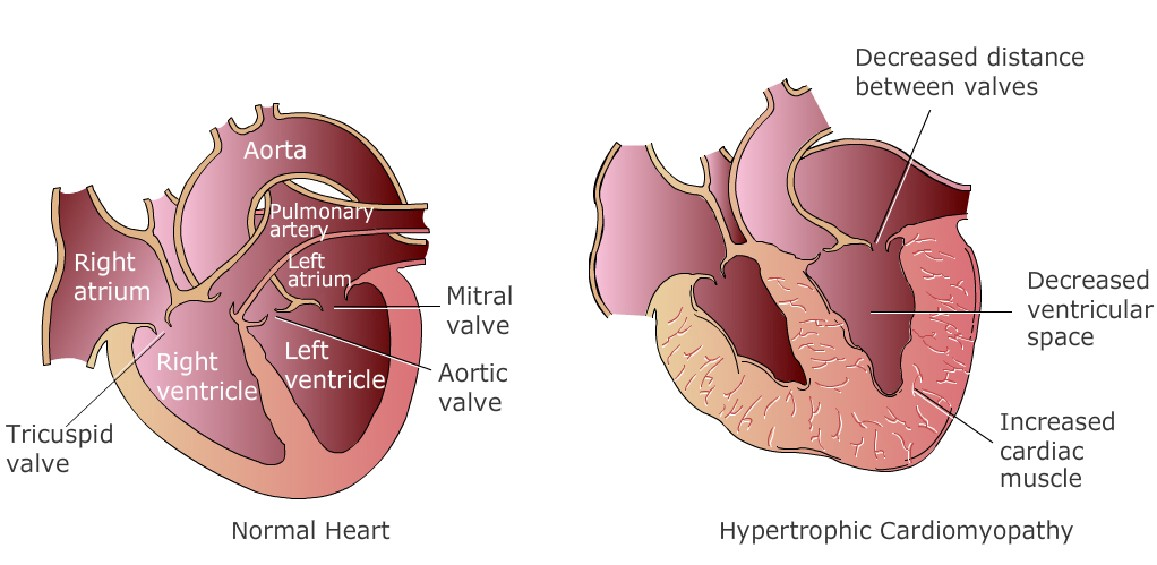
\includegraphics[width=12cm,height=12cm,keepaspectratio]{Background/hypertension.jpeg}
    \caption{The effects of hypertension on the heart \cite{hypertrophic}}
    \label{hypertension}
\end{figure} \noindent Hence it is clear that hypertension is one of the largest motivating factors for this project.

\begin{table}[H]
    \centering
    \caption{Categories of blood pressure in adults \cite{Wang2018} \cite{Simjanoska20181}}
\begin{tabular}{|c|cc|}
\hline
\multirow{2}{*}{\textbf{Blood pressure classification}} & \multicolumn{2}{c|}{\textbf{Blood Pressure (mmHg)}} \\
 & \textbf{Systolic} & \textbf{Diastolic} \\ \hline
Hypotension & $\le$ 90 & Or $\le$ 60 \\
Normal & 90-119 & And 60-79 \\
Prehypertension & 120-139 & Or 80-89 \\
Stage 1 hypertension & 140-159 & Or 90-99 \\
Stage 2 hypertension & $\ge$ 160 & Or $\ge$ 100 \\ 
Isolated Systolic hypertension & $\ge$ 140 & And $<$ 90\\
Hypertensive crisis & $\ge$ 180 & Or $\ge$ 110 \\ \hline
\end{tabular}
\label{bp_vals_table}
\end{table}


\subsubsection{Blood Pressure measurements} 
Blood pressure (BP) is the force of the blood pushing against the 
arterial walls as the heart pumps blood. It is measured in millimeters of 
mercury (mmHg) \cite{Simjanoska20182}. BP  is  measured  in  terms  of  
systolic  blood  pressure  (SBP)  and  diastolic  blood  pressure  
(DBP). These values are the maximum and minimum pressure values of an 
Arterial Blood Pressure waveform during a cardiac cycle 
respectively \cite{Simjanoska20181} \cite{Pradenas2020}. An example of this structure is provided in Figure \ref{abp}.
\begin{figure}[H]
   \centering
   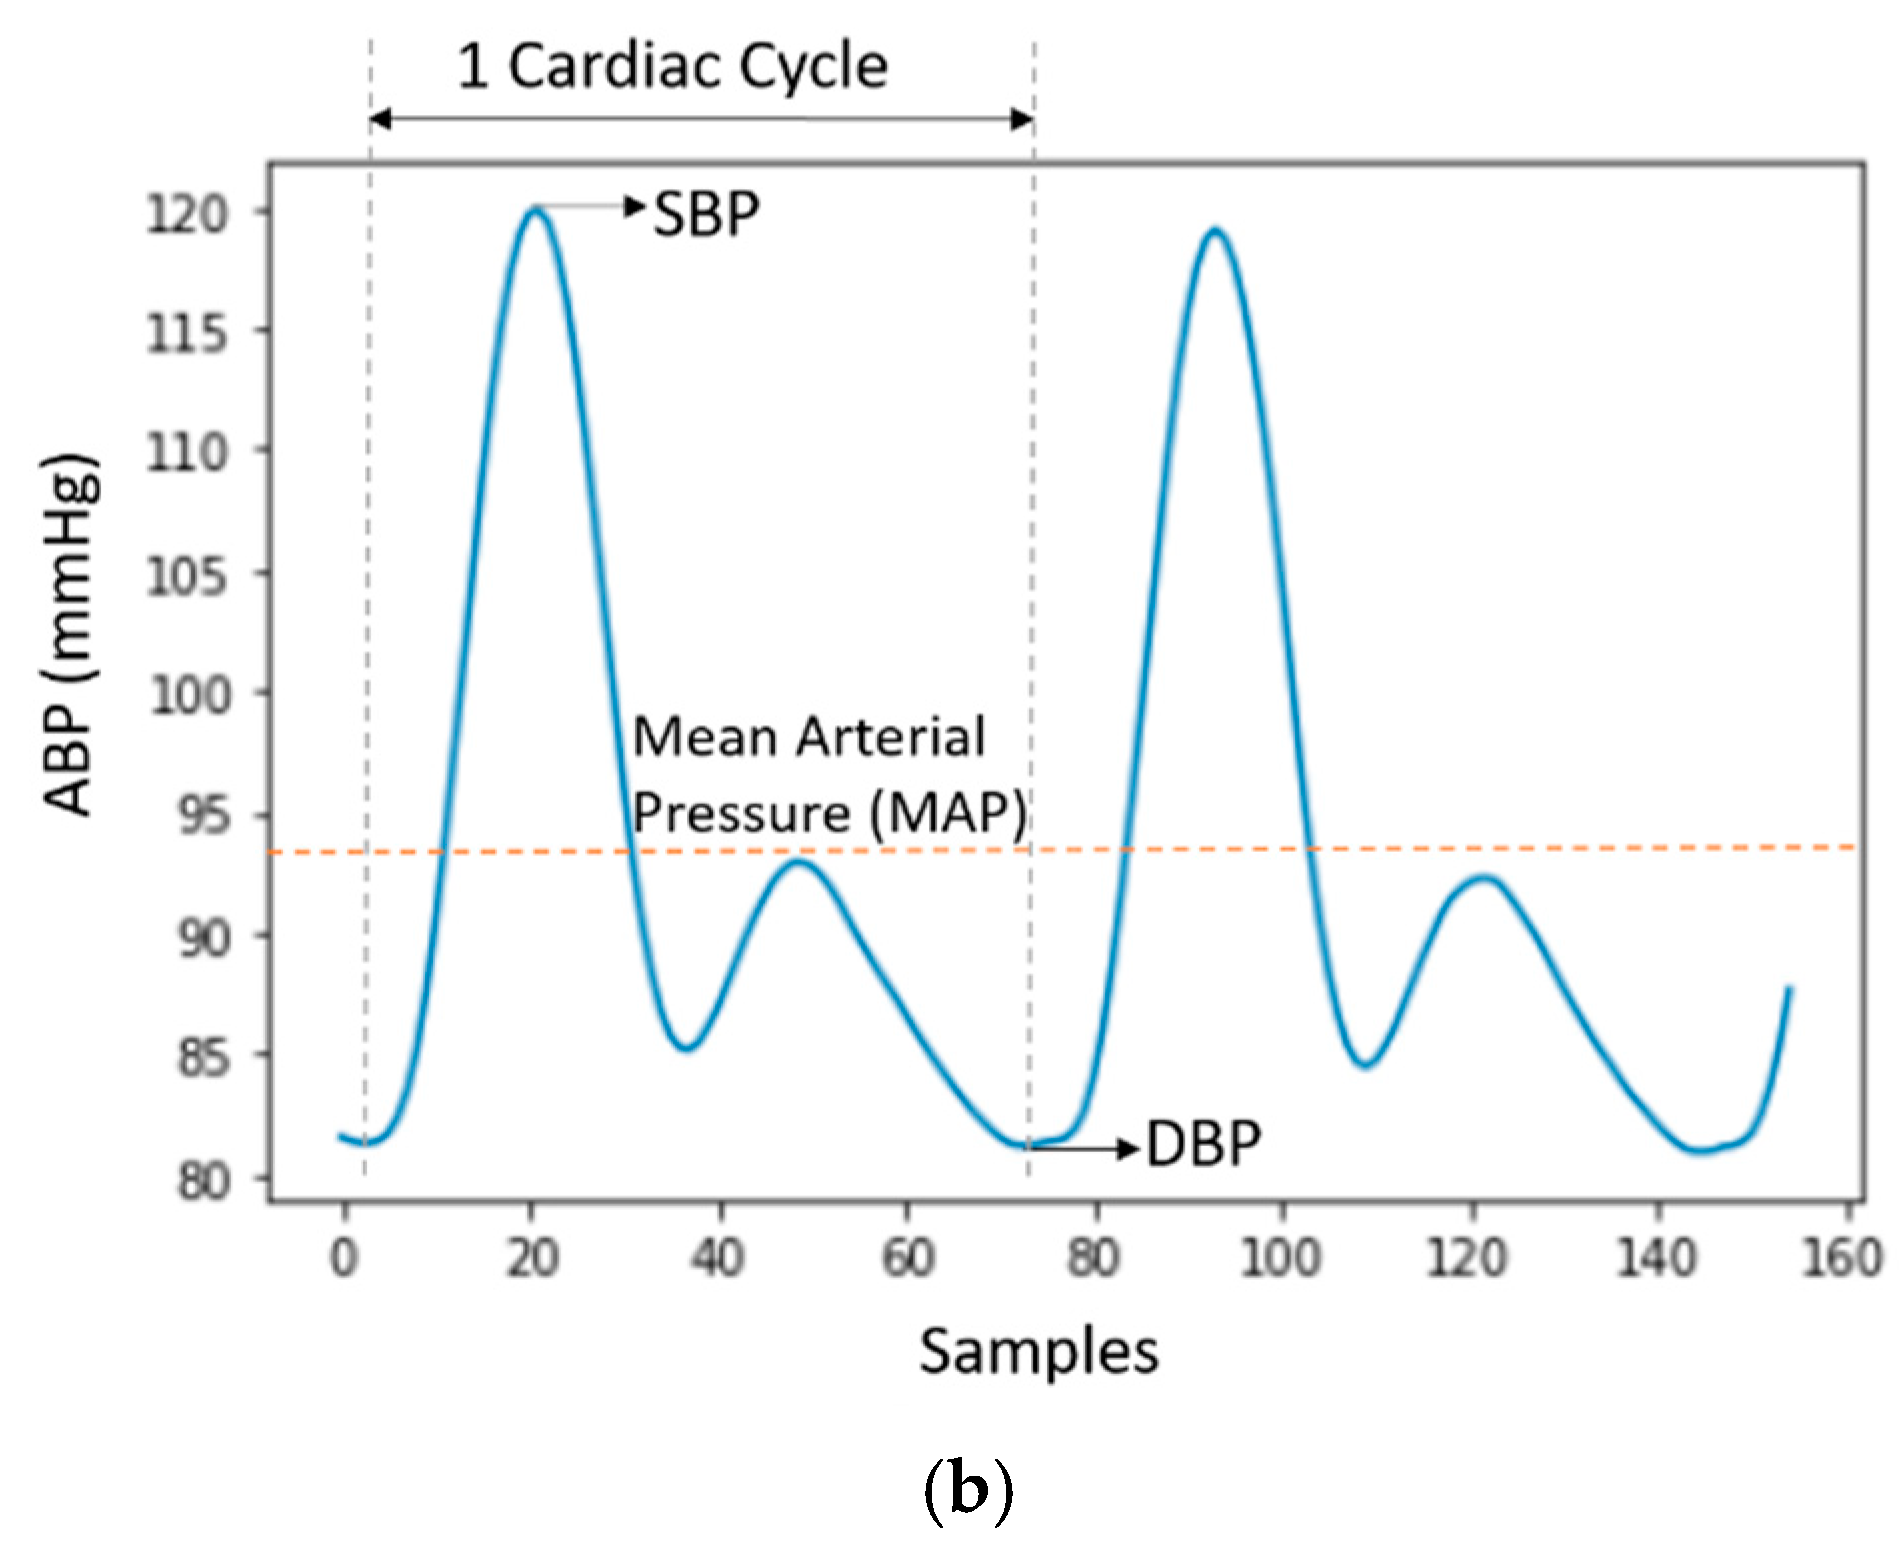
\includegraphics[width=12cm,height=12cm,keepaspectratio]{Background/abp.png}
   \caption{Structure of an Arterial Blood Pressure signal \cite{Athaya2021}}
   \label{abp}
\end{figure}\noindent As shown in Figure \ref{abp}, the Systolic and Diastolic Blood Pressure 
values of the waveform are defined by the maximum and minimum ABP values within the provided 
sampling window. \\ \newline \noindent BP  has 
oscillations or pulses that mirror the oscillatory nature of the heart. The blood is 
propelled during systole, also known as heart contraction, and the blood is  
rested during  diastole, known as heart  relaxation, as illustrated in Figure \ref{diastoleSystole}. \begin{figure}[H]
    \centering
    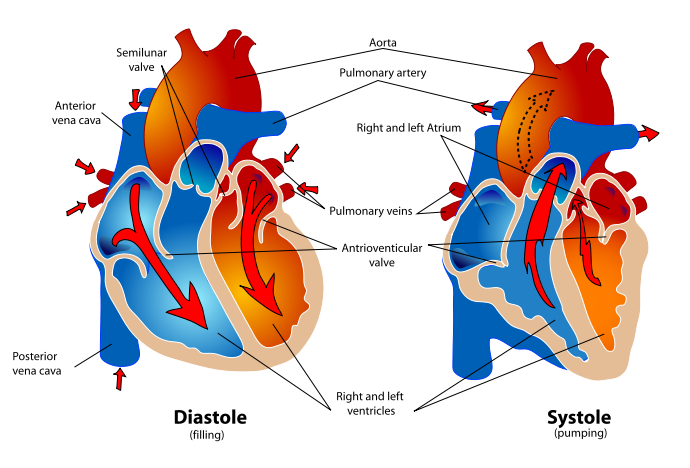
\includegraphics[width=12cm,height=12cm,keepaspectratio]{Background/sbp_dbp.png}
    \caption{Visualisation for SBP and DBP \cite{SBP}}
    \label{diastoleSystole}
\end{figure} \noindent There 
are two  conventional  methods  for  measuring  blood  pressure (BP). These 
are invasive   and   non-invasive methods. \\ \newline \noindent \textcolor{red}{If you're going to use firstly, there should be consistency. I.e where is secondly or finally? Check throughout report.}
Firstly, a description on invasive methods. The most popular form of invasive  BP 
measurement is  catheterization \cite{Zaki2018}. Invasive BP measurements 
are continuous and the most accurate from heartbeat to heartbeat. As a result 
these measurements are recognised as the gold standard 
internationally \cite{Sharma2017} \cite{ElHajj2020}. However, this method is 
usually restricted to hospitals, as medical supervision is required \cite{Pradenas2020}. 
In addition, this method poses several health risks, including bleeding and 
infection. As a result, invasive measurements are only utilised for critically 
ill patients in intensive care units and for use during 
surgery \cite{Zaki2018}\cite{ElHajj2020}. \\ \newline \noindent \textcolor{red}{Check throughout the report: Type in 3rd person and not colloquial/chatty.} Now a description 
on non-invasive methods. The gold standard for BP measurement is the use of a 
cuffed sphygmomanometer. Cuff-based methods provide BP measurements without 
any major side effects as opposed to BP measured invasively \cite{ElHajj2020}. However, 
patients will feel uncomfortable with long term monitoring due to the painful cuff 
inflation which interrupts the regular blood flow \cite{Tanveer2018}. In addition, 
these methods can only measure BP intermittently with intervals between measurements 
greater than at least two minutes. These devices are too cumbersome to wear during 
measurements. Also, it has been found that over three in ten home BP monitoring 
cuffs have produced inaccurate results \cite{Leung2016}. \\ \newline \noindent  As a 
result, the existing invasive and non-invasive BP measurement techniques are not 
feasible for an implementation involving continuous ambulatory BP 
monitoring \cite{ElHajj2020}. Hence, after having assessed the viability of all 
aforementioned methods, it is clear that it is difficult for these methods to be 
integrated with wearable technologies, which continue to gain popularity in 
commercial sectors and clinical practice \cite{Sharma2017}.

\subsubsection{Ambulatory Blood Pressure (ABP)}
ABP monitoring (ABPM) is when BP is measured as the patient moves around, and it allows 
patients to still live their normal daily lives \cite{Huang2021}. It has been 
classed as the gold standard for detecting and diagnosing hypertension and 
also assessing BP values over a 24 hour period \cite{Kario2021}. ABPM provides 
data on several important and unique parameters \cite{Kario2021}. This data can
 explain how changes in your BP may correlate with your daily activities and sleep 
 patterns \cite{Huang2021}. Conventionally,  ABP is monitored by using a cuff 
 attached to a portable device which is worn on the patient's 
 waist \cite{Kario2021}. In the data provided for this project, the blood pressure signals 
 have been recorded from ICU patients. As a result, these waveforms are not ABP waveforms but are 
 instead Arterial Blood Pressure waveforms.



 \subsubsection{Electrocardiogram (ECG) signals} 
 ECG signals provide an overview of the electrical impulses occurring in the 
 heart \cite{Simjanoska20181}. Electrical changes in the heart conduct
  through the body and are received at skin level. The record of these
   electrical fluctuations during the cardiac cycle is called the 
   Electrocardiogram (ECG) \cite{Kumar2015}. The signals are recorded 
   by measuring the electric potential difference by placing electrodes 
   across the heart of an individual \cite{Tanveer2018} \cite{Simjanoska20181}. 
   These electrodes are connected to the ECG machine with recordings from 12 
   different places on the body, which is known as the 12-lead ECG. The standard 
   ECG leads are I, II, III, aVF, aVR, aVL, V1, V2, V3, V4, V5, V6. Leads I, II, 
   III, aVR, aVL, aVF are classed as the limb leads and the others are 
   precordial leads \cite{Tanveer2018}. \\ \newline \noindent The QRS complex 
   of an ECG signal is detailed in Figure \ref{qrs}. This complex is first 
   created through the generation of the electrical impulses from the heart. 
   These signals then move along the electrical highway and as a result cause 
   the ventricles to contract and pump oxygenated blood into the arteries. 
   Physically, this whole describes the QRS 
   complex \cite{Kumar2015}. \begin{figure}[H]
    \centering
    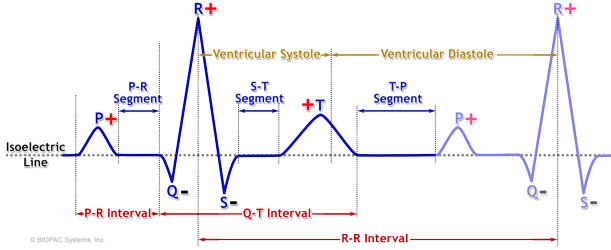
\includegraphics[width=12cm,height=12cm,keepaspectratio]{Background/qrs.png}
    \caption{Structure of an ECG signal \cite{ecgWiki} \cite{qrsWiki}}
    \label{qrs}
\end{figure}



\subsubsection{Photoplethysmography (PPG) signals} 
Photoplethysmography (PPG) measures the blood volume changes per pulse. It is an optical and non-invasive 
technique that can determine a wide range of medical values, including an estimate for BP \cite{ElHajj2020}. 
Physically, the PPG signal is acquired by measuring the optical signal transmitted through or reflected  
from  the  subject's tissue \cite{Tanveer2018}. The PPG sensor consists of two components. The first component 
is an Light Emitting Diode (LED) to light up the surface of the skin. The second component is a photodetector, 
which is utilised for measuring the changes in light absorption over a period of time \cite{ElHajj2020} \cite{Kumar2015}.
\begin{figure}[H]
    \centering
    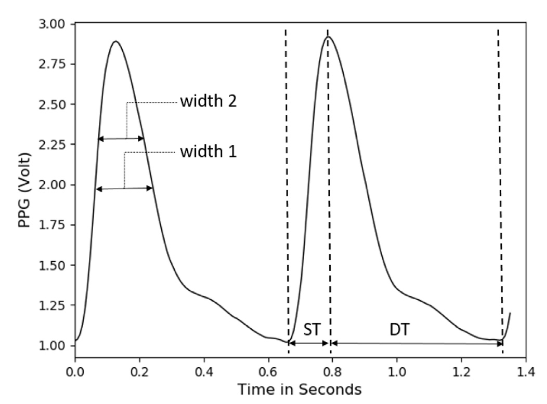
\includegraphics[width=12cm,height=12cm,keepaspectratio]{Background/ppg.png}
    \caption{Structure of a PPG Signal \cite{ElHajj2020}}
    \label{ppg}
\end{figure} \noindent In Figure \ref{ppg}, the four features 
are the Systolic upstroke Time (ST), Diastolic Time (DT), 
width at $\frac{1}{2}$ amplitude (width 1) and width at $\frac{2}{3}$ 
amplitude (width 2) \cite{ElHajj2020}. PPG waveforms have a wide range of 
temporal features \cite{ElHajj2020}. These features have been utilised 
in several experimentations, creating  models  to  estimate blood 
pressure \cite{Pradenas2020}.


\subsection{Cuff-less methods for deriving BP} 
Cuff-less  methods have great potential in being used to estimate BP. 
This is because they provide continuous measurements, they cause minimal 
harm to the patients and they produce BP values over a long period of 
time  \cite{Liu2020}. There are three fundamental cuff-less methods 
which will now be discussed which can be used for deriving BP. These 
three methods rely on Pulse Transit Time (PTT), Pulse Arrival 
Time (PAT) and Pulse Wave Velocity (PWV) respectively \cite{Nye2015}. These 
will each now be discussed in more detail.

\subsubsection{Pulse Transit Time (PTT)} 
PTT is the time required for the arterial pressure wave to travel from the 
left ventricle to a distal arterial site. PTT holds an inverse relationship 
to blood pressure and as a result it is dependent on arterial compliance, 
arterial wall thickness, arterial radius, and blood density. PTT is 
conventionally found with the use of two PPG 
sensors \cite{Tanveer2018} \cite{Wang2018} \cite{ElHajj2020}, as indicated 
in Figure \ref{ptt}.
\begin{figure}[H]
    \centering
    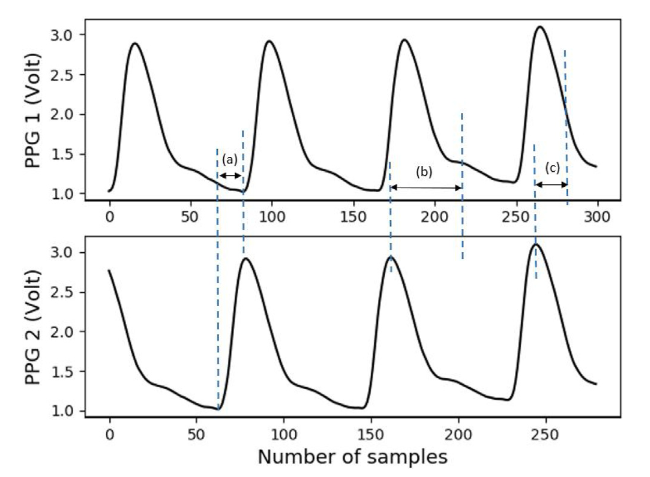
\includegraphics[width=12cm,height=12cm,keepaspectratio]{Background/ptt.png}
    \caption{Pulse Transit Time (PTT) visualisation \cite{ElHajj2020}}
    \label{ptt}
\end{figure} \noindent It is important to note for 
Figure \ref{ptt} that the PTT can be measured at different points along 
the PPG waveforms. (a) represents a foot-to-foot time delay, (b) is a 
peak-to-dicrotic notch time delay and (c) is a peak to mid-point of the 
falling edge time delay \cite{ElHajj2020}. As a proof of concept, increasing 
BP leads to an increase in the tension along the arterial wall tension, which 
therefore reduces the PTT. Hence, the opposite also applies \cite{Kumar2015}.

\subsubsection{Pulse Arrival Time (PAT)} 
The PAT is the difference in time between the R-peak of the ECG signal and 
the systolic peak of the PPG signal when measured during the same 
cardiac cycle, as indicated in 
Figure \ref{pat} \cite{ElHajj2020} \cite{Malikeh2019}. Physically, 
PAT is the interval in time between the activation of electrical 
impulses at the heart and the arrival of the pulse wave at a location 
on the body, such as the finger \cite{Jeong2021}. PAT is measured using 
two sensors, an ECG and a PPG sensor \cite{ElHajj2020}. 
\begin{figure}[H]
    \centering
    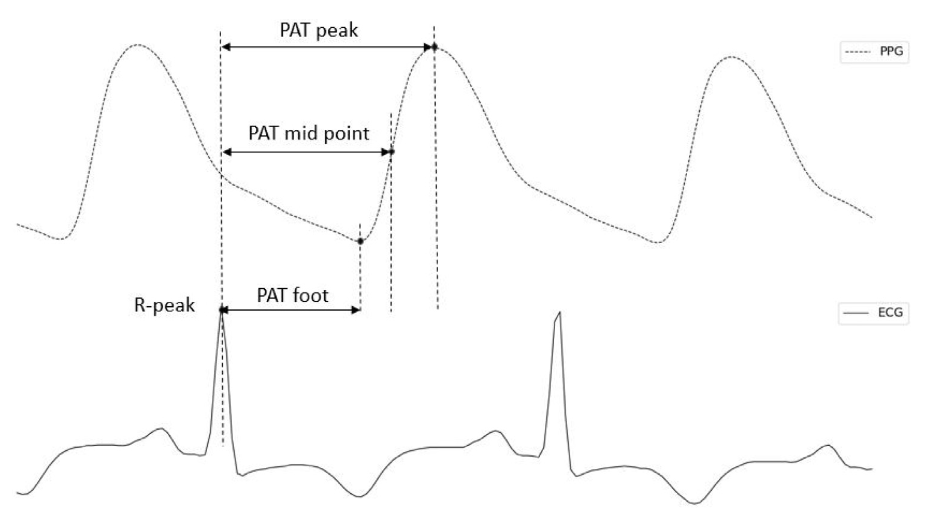
\includegraphics[width=12cm,height=12cm,keepaspectratio]{Background/pat.png}
    \caption{Pulse Arrival Time (PAT) visualisation \cite{ElHajj2020}}
    \label{pat}
\end{figure} \noindent The Pre-ejection Period (PEP) delay can 
also be briefly discussed. PEP is the time needed to convert the electrical 
signal into a mechanical pumping force and isovolumetric contraction to open 
the aortic valves, 
\begin{align}
    PAT = PTT + PEP
\end{align}

\subsubsection{Pulse Wave Velocity (PWV)}
The PWV calculates the velocity of the pulse wave using two PPG sensors 
located on the same arterial branch at a known distance 
apart \cite{Pradenas2020} \cite{ElHajj2020}. The relation between PTT 
and PWV can be expressed as 
\begin{equation}\label{eq_pwv1}
    PWV = \frac{d}{PTT}
\end{equation} where $d$ is the arterial distance travelled by the pressure 
wave. PWV is related to the Young's modulus of the vessel wall by the 
Moens-Kortweg equation, 
\begin{equation}\label{eq_pwv2}
    PWV = \sqrt{\frac{Eh}{\rho d}}
\end{equation} where \\ \newline \noindent 
\begin{flalign}
        PWV &= \text{ Velocity of the pulse wave (m/s)} &\\
        E &= \text{ Young's modulus of vessel wall (Pa)} &\\
        h &= \text{ vessel thickness (m)} &\\
        \rho &= \text{ blood density (kg/$m^3$)} &\\
        d &= \text{ arterial diameter (m)} &
    \end{flalign}\\ \newline \noindent The Young's modulus of the 
vessel wall is then related to the arterial pressure by the 
Bramwell-Hills equation, 
\begin{align}
    E = E_0 e^{\lambda P}
\end{align}where $E_0$ and $\lambda$ depend  on  the  thoracic  and 
abdominal aortas and P is the vessel blood pressure 
(mmHg) \cite{Janjua2017} 
\cite{Tanveer2018} \cite{Yang2020}. \\ \newline \noindent By equating and solving 
Equations \ref{eq_pwv1} and \ref{eq_pwv2}, the final equation for estimated 
blood pressure is expressed as, \begin{align}
    P = \frac{1}{\lambda} \ln{(2 r \rho \frac{\Delta X^2}{E_0 h})} - \frac{2}{\lambda} \ln{(PTT)}
\end{align} \\ \newline \noindent where 
\begin{flalign}
    r &= \frac{d}{2} = \text{ arterial radius} &\\
    \Delta X &= \text{ distance from heart to vessel} &
\end{flalign}

\subsubsection{Limitations}
The blood pressure (BP) can be derived through mathematical models as 
soon as estimates have been calculated for PTT, PAT and PWV. Although 
these models are common approaches for BP monitoring in an environment 
that is non-invasive and cuff-less, there are many challenges to these 
implementations. As a result, none of these techniques by themselves 
have been established as a reliable indicator for the estimation 
of BP. \\ \newline \noindent Firstly, all three of the aforementioned 
methods require two separate measurements from two synchronised sensor 
devices. This can be a very inconvenient process for patients who are
uncomfortable with this method \cite{Jeong2021}. \\ \newline \noindent In 
addition, there is a very likely possibility that these sensor devices 
will have different real-time sampling rates. Their operability depends 
on rather complicated arterial wave propagation 
models \cite{ElHajj2020}. \\ \newline \noindent In order to be able to 
continuously measure BP, constant calibration of the methods is 
required. This is due to individual patients having different 
physiological parameters \cite{Jeong2021}. \\ \newline \noindent Finally, 
even with per-person calibration, these models can only provide BP 
estimation for a short period of time. As a result, this makes the 
models unreliable for the estimation of BP with every 
heartbeat \cite{ElHajj2020}. \\ \newline \noindent To conclude this 
chapter, there is a lot of potential in the use of the three above 
parameters in the estimation of Ambulatory BP. However, there are still 
overarching limitations which currently hinder the progress of these 
parameters. 
%As it will be discussed in Chapter 4, it will be indicated 
%that these parameters still play a role in the estimation process but 
%in methods which are more data driven.




 \subsection{Neural Networks}

 \textcolor{red}{You need an intro for neural networks. Again, you can't assume the reader knows what it is.}

 \textcolor{red}{Include a summary to explain what neural network is, before diving into particular types.}

 \textcolor{red}{Also summarise the type of networks you'll be discussing. You need to improve on organising and structuring here..}

 \subsubsection{Artificial neural networks}
 Due to advancements in technology related to machine learning, there has 
 been a lot of research into neural networks algorithms that can offer 
 continuous BP measurements that are non-invasive and also 
 cuff-less \cite{Pradenas2020}. However, in this case BP 
 estimation is motivated by how much data is available to the 
 algorithm \cite{ElHajj2020}. \\ \newline \noindent Artificial neural 
 networks (ANNs) are a machine learning method that can be used to estimate 
 blood pressure \cite{Pradenas2020}. For this report, the aim is to experiment 
 with Recurrent Neural Networks (TNNs). However, in order to properly understand RNNs, 
 it is necessary to first introduce ANNs. ANNs are based on the neural networks 
 found in the human body and aim to replicate their behaviour \cite{Yang2020}. The 
 structure of the ANN consists of multiple individual units called neurons, as shown in Figure 
 \ref{neuron}.  \begin{figure}[H]
    \centering
    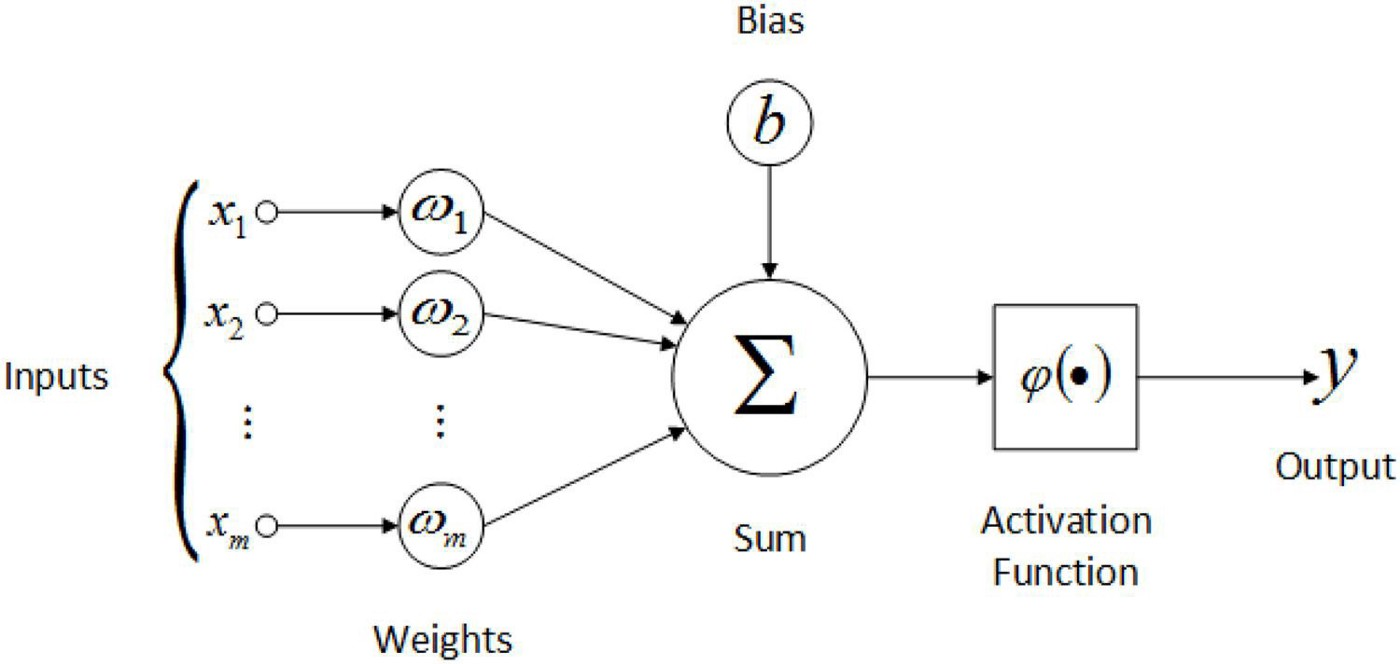
\includegraphics[width=10cm,height=10cm,keepaspectratio]{Background/neuron.jpeg}
    \caption{Structure of a neuron \cite{Almusawi2020}}
    \label{neuron}
\end{figure}\noindent Each 
 neuron has five critical components. These are inputs ($\bm{x}$), weights ($\bm{\omega}$), transfer 
 function ($\Sigma$), activation function ($\phi(\cdot)$) and bias ($b$) \cite{deeplearning}. In order to mathematically 
 express the neuron unit, it is important to first understand its goal. The neuron
 applies a linear transformation to an $m$-dimensional input feature
vector $\mathbf{x}$ by applying a dot product with the weights $\bm{\omega}$ and 
adding a scalar bias $b$ to this dot product. After this, a non-linear 
activation function $\phi(\cdot)$ is applied to the linear mapping. This enables the 
neuron to model non-linear relationships. This is expressed mathematically as follows,
\begin{equation}\label{eq_neuron}
    y = \phi(\sum_{i} \omega_i x_i + b ) = \phi (\bm{\omega}^T \mathbf{x} + b)
\end{equation}\noindent where $\bm{\omega} \in \mathbb{R}^m$ 
and $y$, $b$ are scalars. When each of these neurons are connected together with several other 
neurons across several layers, this forms a neural network, as shown in Figure \ref{ann}. Each of the 
neurons in Figure \ref{neuron} are represented by a grey unit in Figure \ref{ann}.
By having a network of multiple neurons, it is possible to model more 
complex relationships than just a single neuron, provided that the activation functions $\phi(\cdot)$ are not linear for all
neurons (since the combination of linear operations results in a linear operation). In addition,
the output of the neural network can have as many units as needed depending on the task
at hand (e.g. 5 neurons are needed for classification problems with 5 classes using one-hot
encoding).\\ \newline \noindent The network of a single fully-connected layer is mathematically expressed using Equation \ref{eq_layer}, 
\begin{equation}\label{eq_layer}
    \mathbf{y} = \phi (\bm{\Omega} \mathbf{x} + \mathbf{b})
\end{equation}\noindent where $\bm{\Omega} \in \mathbb{R}^{N \times M}$ is the weights matrix, 
$\mathbf{b} \in \mathbb{R}^N$ is the bias vector, $\mathbf{y} \in \mathbb{R}^N$ is the output 
vector and $\phi(\cdot)$ performs element-wise non-linear transformations.

 \begin{figure}[H]
    \centering
    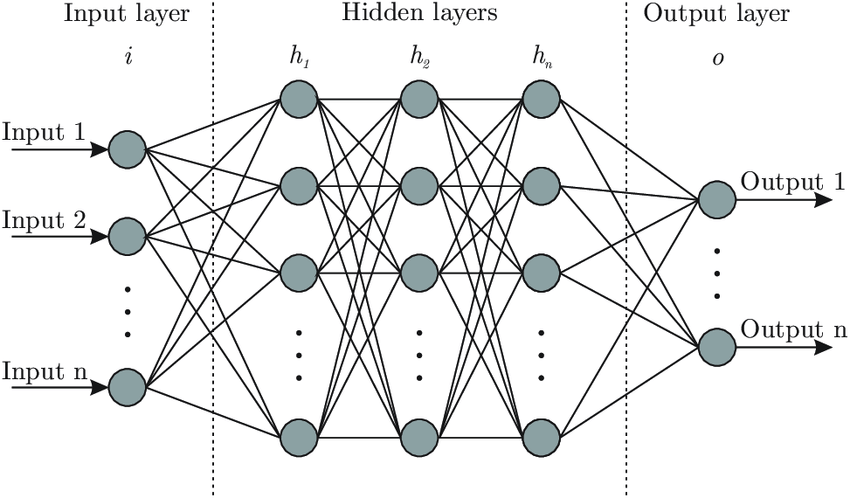
\includegraphics[width=10cm,height=10cm,keepaspectratio]{Background/ann.png}
    \caption{Structure of a multi-layer ANN}
    \label{ann}
\end{figure}

 \subsubsection{Recurrent Neural Networks (RNNs)}
 Traditional neural networks have found success in many fields, However
 it has been demonstrated that they cannot capture
 temporal dependencies in the data, making it unsuitable for signal processing applications. A Recurrent Neural Network (RNN) is a specific type of architecture that is 
 widely used to deal with time-varying data \cite{rnns}. RNNs contain additional memory states that retain and process information from previous
 time steps.\\ \newline \noindent RNNs are called recurrent since 
 they apply the same operation to each of the input sequences, with the output 
 of an individual element being dependent on the previous one. Theoretically, 
 RNNs establish a connection between the actual input and all the previous 
 ones \cite{rnns}. Although this is assumed, in the practice, RNNs have 
 proven to only remember a limited number of inputs. In other words, RNNs 
 have a memory that allows them to remember previous elements and use their 
 information to deal with the current 
 input \cite{deeplearning}. \noindent Figure \ref{rnn2} shows the simplest version 
of an RNN, which can be easily derived from a simple feedforward architecture by 
adding a single loop:
\begin{figure}[H]
    \centering
    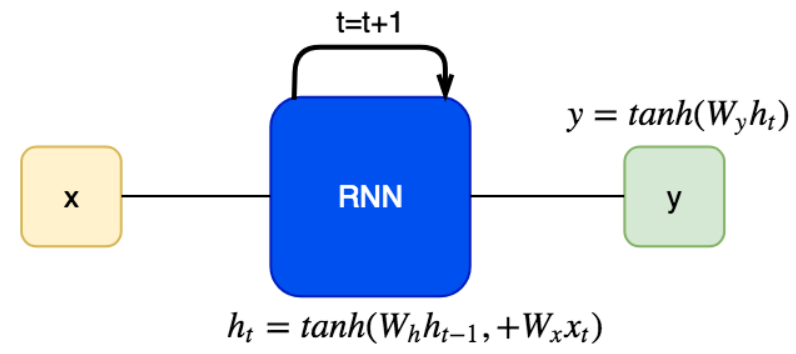
\includegraphics[width=15cm,height=15cm,keepaspectratio]{Background/rnn2.png}
    \caption{Simplification of a RNN}
    \label{rnn2}
\end{figure} \noindent During training, the hidden state $h$ is 
iteratively updated based on the input value $x$ and the learned weights $W_h$  
and $W_x$. The final output $y$  is estimated from the current state $h_t$  
and the matrix $W_y$. Although RNN can assure short-term dependencies within 
the network, simple RNNs become unable to learn to connect information as the 
gap between past and present information grows \cite{lstm}. To overcome this 
limitation, in practical applications LSTM unit is adopted, that is a special 
RNNs architecture composed of multiple interacting layers.
\begin{figure}[H]
    \centering
    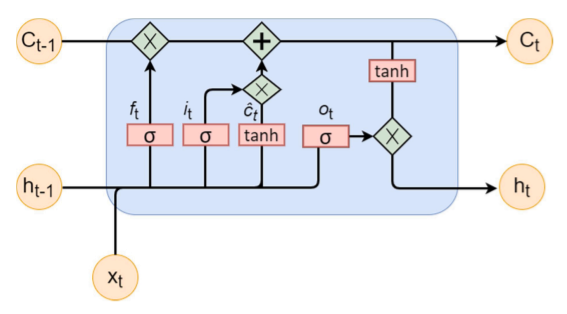
\includegraphics[width=15cm,height=15cm,keepaspectratio]{Background/rnn3.png}
    \caption{LSTM network}
    \label{rnn3}
\end{figure} 

\begin{comment}
     \subsubsection{Transformer Neural Networks (TNNs)}
 RNNs are still quite used in several architectures and Natural Language 
 Processing (NLP) tasks. However the Transformer Neural Network (TNN) 
 has now started to outperform RNNs in several text/NLP benchmarks. 
 A Transformer does not use any recurrence, it instead uses attention 
 to focus on specific parts of a 
 sentence \cite{deeplearning}. \\ \newline \noindent Both text 
 classification and text generation tasks have been successfully 
 tackled by transformers. Transformers seem to scale better than 
 recurrent neural networks. They can have great results when 
 using large architectures and large datasets, whereas RNNs seem 
 not to benefit as much from using more parameters and training 
 examples. State-of-the-art transformer models can have even 
 billions of parameters and can benefit from training in terabytes of 
 text data \cite{deeplearning}. \begin{figure}[H]
    \centering
    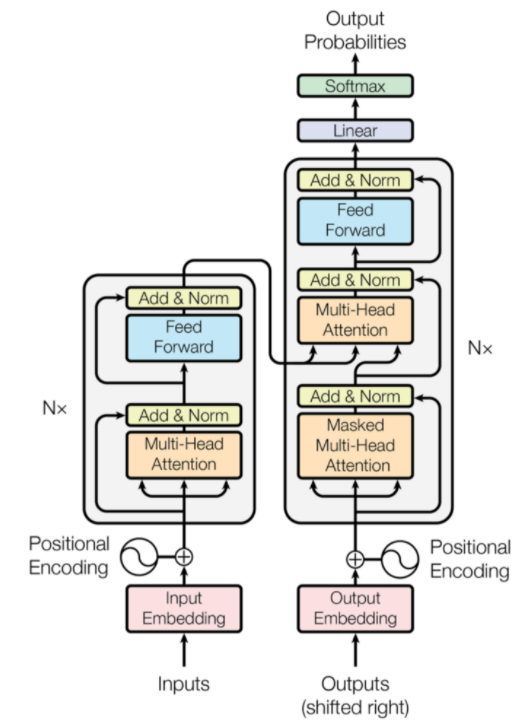
\includegraphics[width=10cm,height=10cm,keepaspectratio]{Background/tnn.png}
    \caption{Model architecture for a transformer}
    \label{tnn}
\end{figure} 

\end{comment}

 \subsubsection{Activation Functions}
 Activation functions transform the output of a neural network unit element-wise, allowing it
to model non-linear functions. For this project, the estimation of BP is treated as a regression problem. 
Hence,

 \subsubsection{Loss Functions}
 Loss functions are objective functions that the neural network aims to minimize when being
trained. For this project, the loss function of concern is the Mean Squared Error (MSE) loss function, which is defined in 
Equation \ref{eq_mse}.
\begin{equation}\label{eq_mse}
    l_\text{MSE }(\mathbf{y}, \mathbf{\hat{y}}) = \frac{1}{N} \sum_{i=1}^N (\mathbf{y}_i - \mathbf{\hat{y}_i})^2
\end{equation}\noindent where $N$ is the number of training examples, $\mathbf{y}_i$ is the target output vector, and $\mathbf{y}_{\hat{y}_i}$ is the predicted output vector.
The MSE is effective for ensuring that the trained model has no outlier predictions 
with huge errors, since the MSE puts larger weight on theses errors due to the squaring 
operation of the function.

 \subsubsection{Neural Network Training}
 In the same manner for any other machine learning algorithm, neural networks aim to learn an underlying pattern
 present in the data by minimizing an error measure defined by a loss function given some
 sample data (a process known as training). Formally, this problem is done by finding the
 optimal weights of the model per layer as defined in Equation \ref{eq_weightOpt}, where $\mathbf{\hat{y}}$ is the estimate of
 the true label $\mathbf{y}$ and $l$ is the loss function.
 \begin{equation}\label{eq_weightOpt}
    \mathbf{\Omega}_{opt} = \arg \min_{\mathbf{\Omega}} \{\mathbb{E}(l(\mathbf{y}, \mathbf{\hat{y}}))\}
 \end{equation}

\textcolor{red}{At the end of this chapter, I advise you to summarise what the reader should take from this chapter. What is the takeaway message and how are you moving forward from this knowledge. Here you restate your aim and objective and how you are going to move forward.}
\textcolor{red}{(The summary should flow into the next chapter)}

\subsection{Overview on Cuff-Less BP device options} 
Wearable technology provides an opportunity for real-time monitoring of human vital signs, thus enabling the
 possibility for preventive, timely notification and real-time diagnosis. Unlike commonly-used BP sensors,
  which demand a specific measurement procedure, modern wearable bio-sensors monitor vital signals online and all
   day long, presenting no additional burden other than wearing the device.  A wide range of wearable 
   devices achieve very positive results, even those wearables which are cheaper in price \cite{Simjanoska20182}. Some
    of the systems developed for the purpose of non-invasive BP monitoring will be discussed in more detail now. 
    In addition, they will be critically analysed against two other viable alternatives. \\ \newline \noindent The 
    motivation behind this project is to replace the current cuff-based BP devices. Cuff-based devices often
     require the supervision of an expert to work correctly and do not provide continuous measurements for BP. 
     In addition they can cause irritation and inconvenience for patients due to cuff inflation and deflation. 
     As a result, current clinical cuff-based BP devices are not suitable for providing continuous BP monitoring 
     which could play a significant role in the early detection of diseases which affect the heart \cite{ElHajj2020}.

\subsubsection{Smart Watches}
Smart watches are becoming an increasingly popular form of wearable technology \cite{Bard2019}. Most of the existing smart
 watch produces currently measure BP through Pulse Transit Time (PTT) from a pulse wave measurement at the wrist. The Heartisans 
 BP smartwatch uses ECG and PPG signals to measure PTT and estimate BP. The watch requires a motionless 20 second scan with 
 the device held at heart level for measurements and provides systolic and diastolic BP readings. Calibration with a
  validated cuff-type BP device is required prior to standalone use. Despite its availability on the market, the 
  Heartisans Watch has not undergone a formal validation study \cite{Bard2019}. \\ \newline \noindent Another wearable 
  method  is  through  arterial  tonometry. The BPro device, developed by the London company HealthSTATS Technologies, 
  is one such device.
\begin{figure}[H]
    \centering
    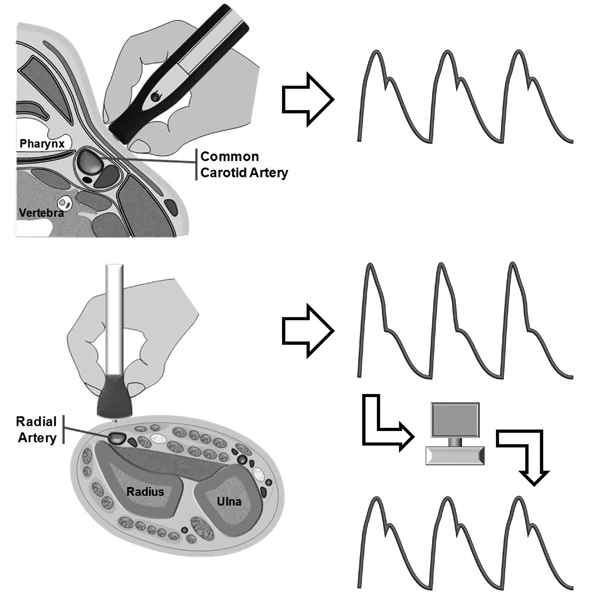
\includegraphics[width=6cm,height=6cm,keepaspectratio]{Background/arterial.png}
    \caption{Arterial Tonometry}
    \label{tonometry}
\end{figure} \noindent Figure \ref{tonometry} shows two different methods for using arterial 
tonometry to measure blood pressure. The first image shows that the recording is taking at the carotid 
artery level in order to estimate the central blood pressure waveform. In the second image, the recording 
is taken at the radial artery level to estimate the arterial pulse wave. The central waveform is then 
reconstructed from this pulse wave using software. \\ \newline \noindent The BPro allows for continuous  24 hour 
 waveform  analysis  of  BP. Calibration to the brachial artery BP is required using a validated upper arm cuff 
 device prior to use. The BPro has been validated in a non-ambulatory study following the Association for the 
 Advancement of Medical Instrumentation (AAMI) standards and the European Society of Hypertension (ESH) protocol.

\subsubsection{Smartphone Applications}
Smartphones offer a great potential to expand the continuous recording of BP if their sensors can be 
correctly utilised \cite{Bard2019}. A formal validation study on one particular iOS application, the Instant 
Blood Pressure app, revealed poor accuracy of BP measurements. Mean absolute differences of 12.4 mmHg for 
systolic BP and 10.1 mmHg for diastolic BP were found between the Instant Blood Pressure application and a
 reference device. This resulted in approximately four out of five hypertensive individuals being falsely classified 
 as normotensive  \cite{Bard2019}. The My BP Lab application measures BP through measurements of Pulse Transit 
 Time (PTT). However, there is currently a lack of experimental data to justify it's dominance in the market.

\subsubsection{Medical Tricorders}
A medical tricorder is a handheld portable device used by consumers to self-diagnose medical conditions and take 
basic vital signs measurements. The   BodiMetrics   Performance   Monitor uses ECG and PPG signal data to estimate
 BP through PTT. The Bodimetrics tricorder obtains measurements with a 20 second scan of the user's fingertip
  at heart level but only provides systolic BP data. This tricorder has a large spread in absolute bias against
   an automated sphygmomanometer, hence it is unlikely to meet formal accuracy and precision 
   standards \cite{Bard2019}. \\ \newline \noindent The FreeScan Personal Cardiovascular Monitor, which is 
   developed by the Taiwanese company Maisense Inc., also estimates BP from PTT. However the device uses a force 
   sensor to capture the systolic arterial waveform rather than PPG. This requires the user to physically apply 
   the force sensor directly to the radial artery for around 10 seconds for measurements. The Freescan device 
   has been verified according to the AAMI protocol \cite{Bard2019}. \\ \newline \noindent The SOMNOtouch
    NIBP is a non-traditional medical tricorder that utilizes PTT data collected in a similar fashion to the
     Bodimetrics Performance Monitor. The device has met the ESH standards, however it begins to lose accuracy 
     for higher SBP and DBP values \cite{Bard2019}.

\subsubsection{Conclusion}
After having discussed three viable devices for cuff-less measurements of BP, it has been finalised that smart 
watches are the most viable option. Whilst existing smart watch devices do suffer from inaccuracies in BP estimation
 due to motion, it is clear that they produce the most acceptable results in line with the AAMI and ESH standards. This 
 chapter can be seen as a forward looking overview of how the estimation methods discussed in this report can be used to
  benefit future products. With regards to this project, this chapter can be treated as a supplementary overview.





\subsection{SECTION CLARIFYING WHAT COMPLEXITY MEANS FOR THIS PROJECT?}

 \subsection{Literature Review}

\textcolor{red}{Initial remarks:Where is the use of the PRISMA criteria? Where is the inclusion, exclusion diagram?}
\textcolor{red}{After reading remarks:}
\textcolor{red}{This is not a literature review. By only placing papers into a table as a summary is not sufficient.}
\textcolor{red}{- what comments do you have on the results you've tabulated?}
\textcolor{red}{- You mention factors were considered.. why? and when you considered them, what about them? Why is it important?}
\textcolor{red}{- What should the reader be left with?}

\textcolor{red}{What are the advantages and disadvantages?}

\textcolor{red}{Currently, the literature review is below average. You need to work on this.}

This chapter provides a detailed account of the literature review conducted for this FYP. 
The literature search equation used will first be discussed, followed by an explanation of the PRISMA 
flow diagram and how it was used to benefit this literature review. To help the reader, 
a table of the scientific papers used in this project is provided. Finally, a critical analysis 
will be given on the literature review and what can be concluded as a result. WHAT DO YOU AIM TO GET OUT OF THIS?

\subsubsection{Survey Equation}
At the beginning of the FYP, the only information provided was the FYP mission statement (see Appendix Item 10.1) and two 
published papers, \emph{A review of machine learning techniques in photoplethysmography for the non-invasive cuff-less measurement of blood pressure} \cite{ElHajj2020} and 
\emph{Continuous Blood Pressure Estimation From Electrocardiogram and Photoplethysmogram During Arrhythmias} \cite{Liu2020}. These resources pserved as an introduction to both the medical background 
and machine learning knowledge for myself. After reviewing this information, the next step was to perform an informal search of literature databases using keywords 
extracted from the FYP brief. These keywords can be divided into two fields: 
\\ \newline \noindent \textbf{Background knowledge}
\begin{itemize}
    \item "Ambulatory"
    \item "Blood Pressure"
    \item "Electrocardiogram"
    \item "Photoplethysmography"
    \item "Wearable technology"
\end{itemize}\noindent \textbf{Implementation strategy}
\begin{itemize}
    \item "Accuracy"
    \item "Algorithm"
    \item "Computational complexity"
\end{itemize}\noindent These keywords were entered into 3 official literature databases, as shown in Table \ref{tabDatabases}.

\begin{table}[H]
    \centering
    \caption{Official online databases used to conduct the literature review \cite{databasesImperial}}
    \label{tabDatabases}
    \resizebox{\columnwidth}{!}{%
    \begin{tabular}{|c|c|}
    \hline
    \textbf{Literature database}          & \textbf{Description}                                           \\ \hline
    ACM Digital Library                   & The digital library of the Association for Computing Machinery \\
    Engineering Village & Database platform for Physics, Electrical Engineering, Electronics and Computing               \\
    IEEE Xplore         & Digital library containing full text of IEEE journals, conference/meeting papers and standards \\
    National Library of Medicine (Pubmed) & Biomedical and life sciences literature                        \\ \hline
    \end{tabular}%
    }
\end{table}\noindent This informal search enabled a clearer understanding of how the relevant published literature phrased their titles. Based on the findings of the informal search, the following 
literature survey search equation was used to identify the literature that best fits the needs of the FYP requirements. The equation chosen was: 

\begin{itemize}
        \item (Extraction OR Estimation OR Review) AND (Blood OR Arterial OR Ambulatory OR Cuffless) AND (Pressure) AND (ECG OR PPG) AND (Machine Learning OR Signal Processing).
\end{itemize}\noindent Hence, this equation was entered into the four databases displayed in Table \ref{tabDatabases}.


\subsubsection{PRISMA checklist}
After applying the chosen equation to the four databases in Table \ref{tabDatabases}, 


the following PRISMA checklist was created:

The papers returned were then filtered 
to only those published between 2012 and 2022, i.e. the last 10 years. As a result the following tables summarise 
the most relevant papers for this project.

\subsubsection{Literature survey table}
As a reference, the original literature survey matrix can be found on 
the Github repository \cite{LitSurvey}. Firstly, in 
Table \ref{litsurveytab}, a simplified literature survey has 
been detailed out for the best performing methods which do not 
employ machine learning methods. 
\begin{table}[H]
\caption{Overview of performance of the best non-invasive non-ML cuff-less methods for measuring BP}
\begin{tabular}{|c|c|c|c|c|c|}
\hline
\textbf{Study} & \textbf{Source} & \textbf{No. Subjects} & \textbf{Age} & \textbf{Implementation} & \textbf{MAE SBP} \\ \hline
\cite{Ahmad2012} & ECG, PTT-CP & 10 & 24-63 & Numerical solution & $\pm 5.93$ \\
\cite{Chen2013} & ECG & 5 & N/A & Analytical solution &  $9 \pm 5.6$\\
\cite{Daimiwal2014} & PPG & 16 & 18-48 & Frequency analysis &  $0.8 \pm  7$\\
\cite{Chan2001} & ECG, PPG, PTT & N/A & N/A & Analytical solution &  $7.49 \pm  8.8$\\
\cite{Yamanaka2016} & PTT & 127 & N/A & Wavelet transforms &  $\pm 7.63$\\
\cite{Ding2016} & PTT, PPG & 27 & 21-29 & Analytical solution &  $-0.37 \pm  5.21$\\ \hline
\end{tabular}
\label{litsurveytab}
\end{table}

\textcolor{red}{Table doesn't fit on the page. Consider either turning it landscape or redesigning the table to fit.}

\textcolor{red}{Redesigning could be making a key for different sources and/or the method. E.g ECG = filled square, PPG = filled circle.}

\textcolor{red}{If you are abbreviating or using symbols, state clearly in your table captions.}

\begin{landscape}
    \begin{table}[H]
        \caption{Overview of performance of  the best non-invasive ML cuff-less methods for measuring BP}
        \begin{tabular}{|c|c|c|c|c|c|}
        \hline
        \textbf{Study} & \textbf{Source} & \textbf{No. Subjects} & \textbf{Age} & \textbf{Method} & \textbf{MAE SBP} \\ \hline
        \cite{Yang2020} & ECG, PPG & 14 males & 17-43 & ANN & $7.99 \pm 10.34$\\
        \cite{Gao2016} & PPG & 65 & 22-65 & Wavelet, SVM & $5.1 \pm 4.34$\\
        \cite{Kachuee2015} & PPG & MIMIC II & Adults & Linear Reg., ANN, SVM &  $13.84\pm  17.56$\\
        \cite{Simjanoska20182} & ECG & 51 & 16-83 & Complexity analysis + ML &  $7.72 \pm  10.22$\\ 
        \cite{Wang2018} & PPG & 72 & N/A & ANN (MLP) & $4.02 \pm 2.79$\\
        \cite{Pradenas2020} & ECG, PPG & MIMIC II & Adults,  neonatal & ANN (150 neurons) & $5.76 \pm 6.39$\\
        \cite{Tanveer2018} & ECG, PPG & 39 & 20-100 & ANN-LSTM & 1.10\\
        \cite{Chen2019} & PTT, ECG, PPG & MIMIC I & N/A & SVM, Lin Reg. & $3.27 \pm 5.52$\\ 
        \cite{Ripoll2019} & PTT & 250 & MIMIC I & ANN-RBM & 3.70\\\hline
        \end{tabular}
        \label{litsurveytab2}
    \end{table}
\end{landscape}

% Please add the following required packages to your document preamble:
% \usepackage{graphicx}
% \usepackage{lscape}
\begin{landscape}
    \begin{table}[H]
    \centering
    \caption{Overview of performance of the best non-invasive non-ML cuff-less methods for measuring BP}
    \label{tabLitSurveyML}
    \resizebox{\textwidth}{!}{%
    \begin{tabular}{ccccccccccccccccccc|}
    \hline
    \multicolumn{1}{|c}{\textbf{Author}} &
      \textbf{Year} &
      \textbf{Signals used} &
      \textbf{Best Method} &
      \textbf{Database} &
      \textbf{Number of subjects} &
      \textbf{Subject characteristics} &
      \textbf{Subject demographics} &
      \textbf{Length of recordings} &
      \textbf{MAE SBP (mmHg)} &
      \textbf{MAE DBP} &
      \textbf{MAD} &
      \textbf{Other accuracies} &
      \textbf{Sampling frequency} &
      \textbf{Preprocessing} &
      \textbf{Signal window length} &
      \textbf{Feature Extraction} &
      \textbf{Complexity} &
      \textbf{Feasibility in wearable context?} \\ \hline
    \multicolumn{1}{|c}{Şentürk   et al.} &
      2018 &
      ECG, PPG &
      Lavenberg-Marquardt ANN &
      MIMIC II &
       &
       &
       &
       &
      N/A &
      N/A &
      N/A &
      \begin{tabular}[c]{@{}c@{}}SBP: Mean ± SD: -0.14 ±   2.55\\      \\      DBP: Mean ± SD: -0.004 ± 1.6\end{tabular} &
      125 &
      Wavelet denoising, median filter,   normalisation &
      10 seconds &
      22-time domain features from ECG   and PPG &
      N/A &
      N/A \\
    \multicolumn{1}{|c}{Nath et   al.} &
      2018 &
      PPG &
      \begin{tabular}[c]{@{}c@{}}Random forest classifier (4 BP classes)\\      Number of estimators = 1000\\ max depth = 30\end{tabular} &
      MIMIC &
      72 (20 chosen) &
       &
       &
       &
      N/A &
      N/A &
      N/A &
      Overall accuracy = 90.8\% &
      125 &
      Normalisation, butterworth band   pass filter with cut off frequency 40Hz &
      \begin{tabular}[c]{@{}c@{}}1 for PPG frequency spectrum, \\ 2   for PPG, first deriv., \\ second deriv., FS first deriv and FS second \\ deriv.\\      \\      Overlap = 0.5 * window lengths above\end{tabular} &
      \begin{tabular}[c]{@{}c@{}}71 statistical features and 12   characteristic features.\\      \\      PPG combined with its first and second derivatives and frequency   spectrum.\\      \\      PPG: 15, PPG first deriv: 14, PPG second deriv: 14, PPG FS: 12, FS FD: 14,   FS SD: 14\end{tabular} &
      N/A &
      N/A \\
    \multicolumn{1}{|c}{Maqsood   et al.} &
      2021 &
      PPG &
      Bi-LSTM &
      \begin{tabular}[c]{@{}c@{}}MIMIC II\\      \\      (also PPG-BP, Guilin People's Hospital, China)\end{tabular} &
      219 &
      Hypertensive and diabetic patients &
      21-86 years &
      N/A &
      \begin{tabular}[c]{@{}c@{}}Time-domain features is best:   \\      \\      3.87 ± 4.79 (Bi-LSTM)\end{tabular} &
      \begin{tabular}[c]{@{}c@{}}Frequency-domain I is best:\\      \\      6.17 ± 5.89 (Bi-LSTM)\end{tabular} &
      N/A &
      N/A &
      125 &
      \begin{tabular}[c]{@{}c@{}}Remove irregular segments and  \\ align PPG+BP. Butterworth bandpass filter, min-max norm.\end{tabular} &
      30 seconds &
      \begin{tabular}[c]{@{}c@{}}Time domain: Cardiac period,   systolic time, diastolic time, pulse area. 10\%, 25\%, 33\%, 50\%, 66\%, 75\% (DW,   DW+SW, DW/SW)\\      \\      Statistical: Skewness, kurtosis, perfusion, MAD, max and min \\      \\      Frequency domain:  Multitaper method\end{tabular} &
      N/A &
      N/A \\
    \multicolumn{1}{|c}{Li et   al.} &
      2021 &
      PPG &
      \begin{tabular}[c]{@{}c@{}}PAT-features\\      \\      Train:Test, 70:30\end{tabular} &
      MIMIC II &
      8000 &
      N/A &
      N/A &
      N/A &
      \begin{tabular}[c]{@{}c@{}}PAT-included features:\\      \\      4.881 ± 5.537\end{tabular} &
      \begin{tabular}[c]{@{}c@{}}PAT-included features:\\      \\      6.887 ± 6.954\end{tabular} &
      N/A &
      N/A &
      N/A &
      N/A &
      40 seconds &
      Semi-classical signal analysis   (SCSA) features, Heart rate, Inflection Point Area (IPA) ratio and width,   Large Artery Stiffness Index (LASI), Augmentation Index (AI), PAT &
      N/A &
      N/A \\
    \multicolumn{1}{|c}{Shimazaki   et al.} &
      2018 &
      PPG, VBP, APG &
      \begin{tabular}[c]{@{}c@{}}Autoencoder, ANN regression\\      \\      Train: Test:Val = 70:15:15\end{tabular} &
      N/A &
      1363 &
      \begin{tabular}[c]{@{}c@{}}687 healthy males, \\ 676 healthy females\end{tabular} &
      \begin{tabular}[c]{@{}c@{}}Male age: 56.5 ± 18.5, male SBP:   128 ± 18.1\\      \\      Female age: 59.9 ± 16.0, female SBP 126 ± 20.5\end{tabular} &
      Seating posture for 5 minutes &
      N/A &
      N/A &
      N/A &
      \begin{tabular}[c]{@{}c@{}}Correlation coefficient =   0.78\\      \\      Standard Deviation = 11.86\end{tabular} &
      N/A &
      N/A &
      N/A &
      100 features from the coupling   signal of the pulse wave and from its first-order differentiation and   second-order differentiation &
      N/A &
      N/A \\
    \multicolumn{1}{|c}{Şentürk   et al.} &
      2018 &
      PPG, ECG &
      2  Bi-LSTM and ReLU &
      MIMIC II &
      N/A &
      N/A &
      N/A &
      N/A &
      N/A &
      N/A &
      N/A &
      \begin{tabular}[c]{@{}c@{}}RMSE SBP: 3.63\\      \\      RMSE DBP: 1.48\end{tabular} &
      N/A &
      Normalisation, segmented by R-R   intervals &
      N/A &
      22 time features, 11 from ECG   and 11 from PPG &
      N/A &
      Yes, by changing the number of   features of the system \\
    \multicolumn{1}{|c}{Xie et   al.} &
      2018 &
      PPG &
      Random Forest &
      University of Queensland Vital Signs Dataset &
      11492 samples &
      N/A &
      N/A &
      N/A &
      N/A &
      N/A &
      \begin{tabular}[c]{@{}c@{}}Random Forest: SBP: 4.21 ±7.59   \\      \\      DBP: 3.24 ± 5.39\end{tabular} &
      N/A &
      N/A &
      N/A &
      10 seconds &
      8 features: Pulse onset,   systolic peak, diastolic peak, dicrotic notch, time and area under PPG curve &
      N/A &
      N/A \\
    \multicolumn{1}{|c}{Li et   al.} &
      2020 &
      PPG, ECG &
      \begin{tabular}[c]{@{}c@{}}Supervised ML.\\      \\      \\      SVM with SCSA features\end{tabular} &
      Pulse Wave Database (PWD), MIMIC II &
      \begin{tabular}[c]{@{}c@{}}\textgreater{}4000 (PWD) and \textgreater{}8000   (MIMIC II)\\      \\      8004 sample size for training and testing\end{tabular} &
      N/A &
      N/A &
      N/A &
      SVM: 7.44 ± 7.37 &
      SVM: 5.09 ± 5.66 &
      N/A &
      N/A &
      125 &
      N/A &
      40 seconds &
      \begin{tabular}[c]{@{}c@{}}SCSA:\\      - Eigenvalues\\      - Systolic invariants\\      - Diastolic invariants\\      - Eigenvalue summation\end{tabular} &
      N/A &
      N/A \\
    \multicolumn{1}{|c}{Wang et   al.} &
      2022 &
      PPG &
      AlexNet &
      UCI ML repository (subset of MIMIC II) &
      11294 segments from 348 records &
      N/A &
      N/A &
      Ranging from 8 - 592 seconds &
      0.00 ± 8.46 &
      -0.04±5.36 &
      N/A &
      N/A &
      125 &
      Remove duplicates, remove patients   saturated amplitudes and discontinuities, two moving average filters &
      10 seconds &
      N/A &
      Minimal complexity, uses short   duration of PPG &
      Yes, by changing the number of   features of the system \\
    \multicolumn{1}{|c}{Kachuee   et al.} &
      2017 &
      ECG, PPG &
      AdaBoost / Random Forest &
      MIMIC II &
      3663 records &
      N/A &
      N/A &
      N/A &
      8.21 ± 5.45 &
      4.31 ± 3.52 &
      N/A &
      Meets AAMI standards &
      125 &
      Wavelet decomposition, zeroing   frequency components, wavelet reconstruction &
      N/A &
      \begin{tabular}[c]{@{}c@{}}Physiological: HR, AI, ASI\\      \\      Dimensionality reduction\end{tabular} &
      N/A &
      N/A \\
    \multicolumn{1}{|c}{Singla   et al.} &
      2020 &
      ECG, PPG &
      Linear Regression &
      No &
      33 &
      19:14 male:female &
      60 ± 10 years &
      Training and validation datasets   of 1.5 minutes each &
      0.2 (LR) &
      0.4 (LR) &
      N/A &
      \begin{tabular}[c]{@{}c@{}}LR: RMSE SBP: 0.26\\      \\      RMSE DBP: 0.65\end{tabular} &
      ECG: 200 Hz, PPG: 75 Hz &
      Wavelet transformation (Haar  wavelet, less complexity) &
      N/A &
      25 each for both ECG and PPG &
      Haar wavelet reduces preprocessing   complexity &
      N/A \\
    \multicolumn{1}{|c}{Sertac   et al.} &
      2020 &
      PPG &
      Linear Support Vector Regression   (LSVR) &
      Guilin University of Electronic   Technology &
      216 &
      N/A &
      21-86 years &
      2.1 seconds (segment length) &
      LSVR: 13.57±3.23 &
      LSVR: 8.30±1.88 &
      N/A &
      N/A &
      1000 Hz &
      4th order Chebyshev-II filter with   cutoffs of 0.5 and 5 Hz, normalisation &
      N/A &
      10: Age, height, weight, SBP,   DBP, BMI, W1, W2, ST, DT &
      N/A &
      N/A \\
    \multicolumn{1}{|c}{Jung et   al.} &
      2019 &
      ECG, PPG, PTT &
      \begin{tabular}[c]{@{}c@{}}Semi-supervised learning\\      \\      Linear Regression\end{tabular} &
      N/A &
      9 males &
      Age: 20-29 &
      N/A &
      225 seconds in total &
      N/A &
      N/A &
      N/A &
      N/A &
      N/A &
      Sallen-key low pass filter &
      N/A &
      PTT, MAP, Pulse Pressure   (difference between SBP and DBP) &
      N/A &
      N/A \\
    \multicolumn{1}{|c}{El Hajj   et al.} &
      2020 &
      PPG &
      \begin{tabular}[c]{@{}c@{}}LSTM (64, 512) and GRUs (128, 256,   512)\\      \\      Training:test:val = 60:20:20\\      \\      Adam optimizer\end{tabular} &
      MIMIC &
      500 record files &
      N/A &
      N/A &
      N/A &
      \begin{tabular}[c]{@{}c@{}}LSTM: 3.23±4.74\\      \\      GRU: 3.25±4.76\end{tabular} &
      \begin{tabular}[c]{@{}c@{}}LSTM: 1.59±1.96\\      \\      GRU: 1.43±1.77\end{tabular} &
      N/A &
      N/A &
      125 &
      \begin{tabular}[c]{@{}c@{}}PPG filters and baseline wandering   removed\\      \\      Irregular and distorted signal segments removed\\      \\      Segments with abnormal HR and BP removed\\      \\      PPG and BP aligned, normalisation\end{tabular} &
      \begin{tabular}[c]{@{}c@{}}3 seconds (21000 segments) \\ and 7 seconds (9000 segments)\end{tabular} &
      7 features (CP, DT, DW10/SW10,   DW25, SW33 + DW33, DW75, SW75+DW75) &
      \begin{tabular}[c]{@{}c@{}}GRUs are less computationally   \\ expensive than LSTMs\end{tabular} &
      N/A \\
    \multicolumn{1}{|c}{Shimazaki   et al.} &
      2019 &
      PPG &
      CNN &
      N/A &
      78 &
      \begin{tabular}[c]{@{}c@{}}45 male, 33 female, \\ Japanese adults\end{tabular} &
      N/A &
      50000 pulse wave data &
      N/A &
      N/A &
      N/A &
      \begin{tabular}[c]{@{}c@{}}CNN with pulse wave:\\      \\      R = 0.71, SD = 11.40\end{tabular} &
      1000 Hz &
      4th order Butterworth filter,   cutoff frequency of 30 Hz &
      N/A &
      Only pulse wave feature used in   best method &
      N/A &
      Potentially \\
    \multicolumn{1}{|c}{Yan et   al.} &
      2019 &
      ECG, PPG &
      Multi-task learning CNN &
      MIMIC II &
      604 &
      N/A &
      N/A &
      Each recording is longer than 10   minutes &
      3.09±2.76 &
      2.11±2 &
      N/A &
      N/A &
      125 &
      \begin{tabular}[c]{@{}c@{}}2 mean filters remove motion   artifacts and HF noise from PPG+ECG\\      \\      SBP: 80-180, DBP: 50-130\\      \\      Duration of each record longer than 10 minutes\end{tabular} &
      10 &
      Automatic feature extraction &
      N/A &
      N/A \\
     &
       &
       &
       &
       &
       &
       &
       &
       &
       &
       &
       &
       &
       &
       &
       &
       &
       &
       \\ \hline
    \end{tabular}%
    }
    \end{table}
    \end{landscape}

\subsubsection{Critical analysis of literature survey table}

\subsubsection{Conclusions of literature survey}

The Mean Absolute Error (MAE) of the Systolic BP (SBP) was used as the uniting accuracy measure in this paper, as it was the most readily available parameter in all of the aforementioned papers. \\ \newline \noindent It is important to note that other factors were considered in this literature survey. These factors were, \begin{itemize}
    \item Range of SBP and DBP values 
    \item Sampling frequency
    \item Denoising and detection techniques used
    \item Computational complexity
    \item Feasibility in a wearable context
\end{itemize}\noindent However, due to a lack of regular occurrences of these factors over all the papers, they were not included in the above two tables.\\ \newline \noindent The results show that the established non-ML methods do produce MAE values noticeably lower than the majority of the ML methods. However, a main factor to consider about these results is that machine learning based methods and neural networks are data driven. As shown in Table \ref{litsurveytab2}, there is a very limited number of subjects available for each study. If these studies had been extended to include more test patients, it is possible that these MAE SBP values were lower. An additional point is that another study \cite{Su2017} did a study into using a 4-layer LSTM architecture to estimate BP from ECG and PPG signals with 84 patients. This study resulted in an RMSE SBP of $3.9$ mmHg but no available MAE. Hence there is a lot of potential in ML methods when there is sufficient data available.